% -----------------------------*- LaTeX -*------------------------------
\documentclass[UTF8]{report}
% ------------------------------------------------------------------------
% Packages
% ------------------------------------------------------------------------
\usepackage{ctex}
\usepackage[body={7in, 9in},left=1in,right=1in]{geometry}
\usepackage{amsmath,amsfonts,amssymb,bm,amsthm}%数学宏包、数学字体、数学符号、支持 \mathscr{} 字体、支持粗斜体 \bm{}、数学定理
\usepackage{graphicx}%支持 \includegraphics{} 插图
\usepackage{subfigure}%插入子图
\usepackage{nicefrac}
\usepackage{mathrsfs}
\usepackage{caption}
\usepackage{algorithm,algorithmicx}
\usepackage[noend]{algpseudocode}
\usepackage{fancyhdr}
\usepackage{adjustbox}
\usepackage{esint}%支持多种积分算子
\usepackage{mathtools}%数学宏包的重要补充
\usepackage{upgreek}%数学环境的直立希腊字母
\usepackage{enumitem}%自定义列表环境
\usepackage{color}%支持颜色改变
\usepackage{extarrows}%任意长度的箭头
\usepackage{tikz,xcolor}%画图、画 Feynman 图
\usepackage{breqn}
\usepackage{fontsize}
\usepackage[framemethod=TikZ]{mdframed}
\usepackage{fontspec}
\usepackage{bigstrut,multirow,rotating}%Excel表格自动导入latex
\usepackage{booktabs}
\usepackage{scribe}
% ------------------------------------------------------------------------
% Macros
% ------------------------------------------------------------------------
%~~~~~~~~~~~~~~~
% Utility latin
%~~~~~~~~~~~~~~~
\newcommand{\ie}{\textit{i.e.}}
\newcommand{\eg}{\textit{e.g.}}
%~~~~~~~~~~~~~~~
% Environment shortcuts
%~~~~~~~~~~~~~~~
\newcommand{\balign}[1]{\ealign{\begin{align}#1\end{align}}}
\newcommand{\baligns}[1]{\ealigns{\begin{align*}#1\end{align*}}}
\newcommand{\bitemize}[1]{\eitemize{\begin{itemize}#1\end{itemize}}}
\newcommand{\benumerate}[1]{\eenumerate{\begin{enumerate}#1\end{enumerate}}}
%~~~~~~~~~~~~~~~
% Text with quads around it
%~~~~~~~~~~~~~~~
\newcommand{\qtext}[1]{\quad\text{#1}\quad}
%~~~~~~~~~~~~~~~
% Shorthand for math formatting
%~~~~~~~~~~~~~~~
\newcommand{\mbb}[1]{\mathbb{#1}}
\newcommand{\mbi}[1]{\boldsymbol{#1}} % Bold and italic (math bold italic)
\newcommand{\mbf}[1]{\mathbf{#1}}
\newcommand{\mc}[1]{\mathcal{#1}}
\newcommand{\mrm}[1]{\mathrm{#1}}
\newcommand{\tbf}[1]{\textbf{#1}}
\newcommand{\tsc}[1]{\textsc{#1}}
%\def\<{{\langle}}
%\def\>{{\rangle}}
\newcommand{\sT}{\sf T}
\newcommand{\grad}{\nabla}
\newcommand{\Proj}{\Pi}
%~~~~~~~~~~~~~~~
% Common sets 定义数集符号
%~~~~~~~~~~~~~~~
\newcommand{\R}{\mathbb{R}}
\newcommand{\Z}{\mathbb{Z}}
\newcommand{\Q}{\mathbb{Q}}
\newcommand{\N}{\mathbb{N}}
\newcommand{\C}{\mathbb{C}}
\newcommand{\reals}{\mathbb{R}} % Real number symbol
\newcommand{\integers}{\mathbb{Z}} % Integer symbol
\newcommand{\rationals}{\mathbb{Q}} % Rational numbers
\newcommand{\naturals}{\mathbb{N}} % Natural numbers
\newcommand{\complex}{\mathbb{C}} % Complex numbers
%~~~~~~~~~~~~~~~
% Common functions
%~~~~~~~~~~~~~~~
\renewcommand{\exp}[1]{\operatorname{exp}\left(#1\right)} % Exponential
\newcommand{\indic}[1]{\mbb{I}\left(#1\right)} % Indicator function
\newcommand{\indicsub}[2]{\mbb{I}_{#2}\left(#1\right)} % Indicator function
\newcommand{\argmax}{\mathop\mathrm{arg\, max}} % Defining math symbols
\newcommand{\argmin}{\mathop\mathrm{arg\, min}}
\renewcommand{\arccos}{\mathop\mathrm{arccos}}
\newcommand{\dom}{\mathop\mathrm{dom}} % Domain
\newcommand{\range}{\mathop\mathrm{range}} % Range
\newcommand{\diag}{\mathop\mathrm{diag}}
\newcommand{\tr}{\mathop\mathrm{tr}}
\newcommand{\abs}{\mathop\mathrm{abs}}
\newcommand{\card}{\mathop\mathrm{card}}
\newcommand{\sign}{\mathop\mathrm{sign}}
\newcommand{\prox}{\mathrm{prox}} % prox
\newcommand{\rank}[1]{\mathrm{rank}(#1)}
\newcommand{\supp}[1]{\mathrm{supp}(#1)}
\newcommand{\norm}[1]{\lVert#1\rVert}
%~~~~~~~~~~~~~~~
% Common probability symbols
%~~~~~~~~~~~~~~~
\newcommand{\family}{\mathcal{P}} % probability family / statistical model
\newcommand{\iid}{\stackrel{\mathrm{iid}}{\sim}}
\newcommand{\ind}{\stackrel{\mathrm{ind}}{\sim}}
\newcommand{\E}{\mathbb{E}} % Expectation symbol
\newcommand{\Earg}[1]{\E\left[#1\right]}
\newcommand{\Esubarg}[2]{\E_{#1}\left[#2\right]}
\renewcommand{\P}{\mathbb{P}} % Probability symbol
\newcommand{\Parg}[1]{\P\left(#1\right)}
\newcommand{\Psubarg}[2]{\P_{#1}\left[#2\right]}
%\newcommand{\Cov}{\mrm{Cov}} % Covariance symbol
%\newcommand{\Covarg}[1]{\Cov\left[#1\right]}
%\newcommand{\Covsubarg}[2]{\Cov_{#1}\left[#2\right]}
%\newcommand{\model}{\mathcal{P}} % probability family / statistical model
%~~~~~~~~~~~~~~~
% Distributions
%~~~~~~~~~~~~~~~
%\newcommand{\Gsn}{\mathcal{N}}
%\newcommand{\Ber}{\textnormal{Ber}}
%\newcommand{\Bin}{\textnormal{Bin}}
%\newcommand{\Unif}{\textnormal{Unif}}
%\newcommand{\Mult}{\textnormal{Mult}}
%\newcommand{\NegMult}{\textnormal{NegMult}}
%\newcommand{\Dir}{\textnormal{Dir}}
%\newcommand{\Bet}{\textnormal{Beta}}
%\newcommand{\Gam}{\textnormal{Gamma}}
%\newcommand{\Poi}{\textnormal{Poi}}
%\newcommand{\HypGeo}{\textnormal{HypGeo}}
%\newcommand{\GEM}{\textnormal{GEM}}
%\newcommand{\BP}{\textnormal{BP}}
%\newcommand{\DP}{\textnormal{DP}}
%\newcommand{\BeP}{\textnormal{BeP}}
%\newcommand{\Exp}{\textnormal{Exp}}
%~~~~~~~~~~~~~~~
% Theorem-like environments
%~~~~~~~~~~~~~~~
%\theoremstyle{definition}
%\newtheorem{definition}{Definition}
%\newtheorem{example}{Example}
%\newtheorem{problem}{Problem}
%\newtheorem{lemma}{Lemma}
%~~~~~~~~~~~~~~~
% 组合数学的模板和作业里用到的一些宏包和自定义命令
%~~~~~~~~~~~~~~~
\renewcommand{\emph}[1]{\begin{kaishu}#1\end{kaishu}}
\newcommand{\falfac}[1]{^{\underline{#1}}}
\newcommand{\binomfrac}[2]{\frac{#1^{\underline{#2}}}{#2!}}
\newcommand{\ceil}[1]{\left\lceil #1 \right\rceil}
\newcommand{\floor}[1]{\left\lfloor #1 \right\rfloor}
\newcommand{\suminfty}[2]{\sum_{#1=#2}^{\infty}}
\newcommand{\suminftyk}[0]{\sum_{k=0}^{\infty}}
\newcommand{\sumint}[3]{\sum_{#1=#2}^{#3}}
\newcommand{\sumintk}[2]{\sum_{k=#1}^{#2}}
\newcommand{\suminti}[2]{\sum_{i=#1}^{#2}}
%~~~~~~~~~~~~~~~
% 定义新命令
%~~~~~~~~~~~~~~~
\newcommand*{\unit}[1]{\mathop{}\!\mathrm{#1}}
\newcommand*{\dif}{\mathop{}\!\mathrm{d}}%微分算子 d
\newcommand*{\pdif}{\mathop{}\!\partial}%偏微分算子
\newcommand*{\cdif}{\mathop{}\!\nabla}%协变导数、nabla 算子
\newcommand*{\laplace}{\mathop{}\!\Delta}%laplace 算子
\newcommand*{\deriv}[2]{\frac{\mathrm{d} #1}{\mathrm{d} {#2}}}
\newcommand*{\derivh}[3]{\frac{\mathrm{d}^{#1} #2}{\mathrm{d} {#3^{#1}}}}
\newcommand*{\pderiv}[2]{\frac{\partial #1}{\partial {#2}}}
\newcommand*{\pderivh}[3]{\frac{\partial^{#1} #2}{\partial {#3^{#1}}}}
\newcommand*{\dderiv}[2]{\dfrac{\mathrm{d} #1}{\mathrm{d} {#2}}}
\newcommand*{\dderivh}[3]{\dfrac{\mathrm{d}^{#1} #2}{\mathrm{d} {#3^{#1}}}}
\newcommand*{\dpderiv}[2]{\dfrac{\partial #1}{\partial {#2}}}
\newcommand*{\dpderivh}[3]{\dfrac{\partial^{#1} #2}{\partial {#3^{#1}}}}
\newcommand{\me}[1]{\mathrm{e}^{#1}}%e 指数
\newcommand{\mi}{\mathrm{i}}%虚数单位
%\newcommand{\mc}{\mathrm{c}}%光速 定义与mathcal冲突
\newcommand{\red}[1]{\textcolor{red}{#1}}
\newcommand{\blue}[1]{\textcolor{blue}{#1}}
%\newcommand{\Rome}[1]{\setcounter{rome}{#1}\Roman{rome}}
%~~~~~~~~~~~~~~~
% 一些数学的环境设置
%~~~~~~~~~~~~~~~
%\newcounter{counter_exm}\setcounter{counter_exm}{1}
%\newcounter{counter_prb}\setcounter{counter_prb}{1}
%\newcounter{counter_thm}\setcounter{counter_thm}{1}
%\newcounter{counter_lma}\setcounter{counter_lma}{1}
%\newcounter{counter_dft}\setcounter{counter_dft}{1}
%\newcounter{counter_clm}\setcounter{counter_clm}{1}
%\newcounter{counter_cly}\setcounter{counter_cly}{1}
%\newtheorem{theorem}{{\hskip 1.7em \bf 定理}}
%\newtheorem{lemma}[theorem]{\hskip 1.7em 引理}
%\newtheorem{proposition}[theorem]{Proposition}
%\newtheorem{claim}[theorem]{\hskip 1.7em 命题}
%\newtheorem{corollary}[theorem]{\hskip 1.7em 推论}
%\newtheorem{definition}[theorem]{\hskip 1.7em 定义}
\newcommand{\problem}[1]{{\setlength{\parskip}{10pt}\noindent \bf{#1}}}
\newenvironment{solution}{{\noindent\hskip 2em \bf 解 \quad}}{}
\renewenvironment{proof}{{\setlength{\parskip}{7pt}\noindent\hskip 2em \bf 证明 \quad}}{\hfill$\qed$\par}
%\newenvironment{example}{{\noindent\hskip 2em \bf 例 \arabic{counter_exm}\quad}}{\addtocounter{counter_exm}{1}\par}
%\newenvironment{concept}[1]{{\bf #1\quad} \begin{kaishu}} {\end{kaishu}\par}

% ----------------------------------------------------------------------
% Header information
% ------------------------------------------------------------------------

\begin{document}

\course{B0911005Y-01} 			%optional
\coursetitle{Introduction to Theory of Computation}	%optional
\semester{2023 Spring}		%optional
\lecturer{Mingji Xia}	%optional
\scribe{吉骏雄}		%required
\lecturenumber{2}			%required (must be a number)
\lecturedate{March 24}	%required (omit year)

\maketitle

% ----------------------------------------------------------------------
% Body of the document
% ------------------------------------------------------------------------


\textbf{第2.1次作业: 2.1(c), 2.4(b), 2.6(b), 2.14.}

\problem{2.1} 回忆一下例2.3中给出的CFG $G_4$。为方便起见,用单字母重新命名它的变元如下:
\begin{gather*}
    E \rightarrow E+T       \mid T\\
    T \rightarrow T\times F \mid F\\
    F \rightarrow (E) \mid a
\end{gather*}
给出下述字符串的语法分析树和派生:

\problem{c.} $a+a+a$

\begin{solution}
    语法分析树如图\Ref{fig:2_1}
    \begin{figure}[!htbp]
        \centering
        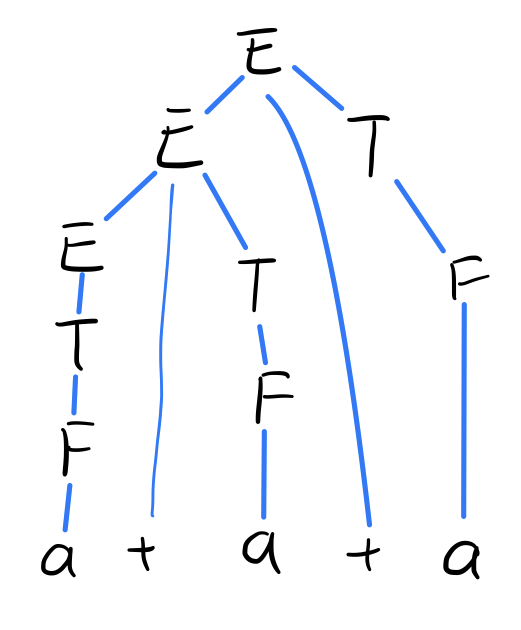
\includegraphics[width=3cm]{image/2.1.png}
        \caption{2.1 c.语法分析树}
        \label{fig:2_1}
    \end{figure}
    派生如下:
    \begin{align*}
        E &\Rightarrow E+T \Rightarrow E+T+T \Rightarrow T+T+T \Rightarrow F+T+T \Rightarrow a+T+T \\
        &\Rightarrow a+F+T \Rightarrow a+a+T \Rightarrow a+a+F \Rightarrow a+a+a
    \end{align*}
\end{solution}


\problem{2.4} 设字母表$\Sigma$是$\{0,1\}$,给出产生下述语言的上下文无关文法:

\problem{b.} $\{ \omega \mid \omega\text{ 以相同的符号开始和结束}\}$

\begin{solution}
    认为空串不属于这个语言的话, 那么文法应该是:
    \begin{align*}
        &E \rightarrow 0F0       \mid 1F1 \mid 0 \mid 1\\
        &F \rightarrow 0F \mid 1F \mid \varepsilon
    \end{align*}
\end{solution}

\problem{2.6} 给出产生下述语言的上下文无关文法:

\problem{b.} 语言$\{a^n b^n \mid n\geq 0\}$的补集

\begin{solution}
    如果一个字符串$\omega$属于它的补集, 那么$\omega$一定满足四种形式之一:
    \begin{enumerate}
        \item 不包含$b$, 即$a^m$或空串$\varepsilon$.
        \item 以$b$开头.
        \item 以$a^{r+s}b^sa$开头, 或就是$a^{r+s}b^s$, 其中$r,s>0$.
        \item 以$a^rb^{r+1}$开头, 其后可能是空串, 也可能不是.
    \end{enumerate}
    因此, 可以给出如下的上下文无关文法:
    \begin{align*}
        &S \rightarrow A\mid B\mid C\mid D\\
        &A \rightarrow aA \mid \varepsilon\\
        &B \rightarrow bR\\
        &C \rightarrow aAGaR \mid aAG\\
        &D \rightarrow GbR\\
        &G \rightarrow aGb \mid ab\\
        &R \rightarrow aR \mid bR \mid \varepsilon
    \end{align*}
\end{solution}


\problem{2.14} 用定理2.6中给出的过程,把下述CFG转换成等价的乔姆斯基范式文法。
\begin{align*}
    &A \rightarrow BAB \mid B \mid \varepsilon\\
    &B \rightarrow 00 \mid \varepsilon
\end{align*}

\begin{solution}
    变化过程如下:
    \begin{enumerate}
        \item 添加新起始变元
        \begin{align*}
            &S_0 \rightarrow A\\
            &A \rightarrow BAB \mid B \mid \varepsilon\\
            &B \rightarrow 00 \mid \varepsilon
        \end{align*}
        \item 删除$B\rightarrow \varepsilon$
        \begin{align*}
            &S_0 \rightarrow A\\
            &A \rightarrow BAB \mid B \mid \varepsilon \mid AB \mid BA \mid A\\
            &B \rightarrow 00
        \end{align*}
        \item 删除$A\rightarrow \varepsilon \mid A$
        \begin{align*}
            &S_0 \rightarrow A \mid \varepsilon\\ 
            &A \rightarrow BAB \mid B \mid AB \mid BA \mid BB\\
            &B \rightarrow 00
        \end{align*}
        \item 删除$A\rightarrow B$
        \begin{align*}
            &S_0 \rightarrow A \mid \varepsilon\\ 
            &A \rightarrow BAB \mid AB \mid BA \mid BB \mid 00\\
            &B \rightarrow 00
        \end{align*}
        \item 删除$A\rightarrow BAB$
        \begin{align*}
            &S_0 \rightarrow A \mid \varepsilon\\ 
            &A \rightarrow CB \mid AB \mid BA \mid BB \mid 00\\
            &B \rightarrow 00\\
            &C \rightarrow BA
        \end{align*}
        \item 删除$S_0\rightarrow A$
        \begin{align*}
            &S_0 \rightarrow CB \mid AB \mid BA \mid BB \mid 00 \mid \varepsilon\\ 
            &A \rightarrow CB \mid AB \mid BA \mid BB \mid 00\\
            &B \rightarrow 00\\
            &C \rightarrow BA
        \end{align*}
        \item 删除$S_0\rightarrow 00, A\rightarrow 00, B\rightarrow 00$
        \begin{align*}
            &S_0 \rightarrow CB \mid AB \mid BA \mid BB \mid ZZ \mid \varepsilon\\ 
            &A \rightarrow CB \mid AB \mid BA \mid BB \mid ZZ\\
            &B \rightarrow ZZ\\
            &C \rightarrow BA\\
            &Z \rightarrow 0
        \end{align*}
    \end{enumerate}
\end{solution}




\textbf{第2.2次作业: 2.11.}

\problem{2.11} 用定理2.12中给出的过程, 把练习2.1中的CFG$G_4$转换成等价的PDA.

\begin{solution}
    结果如图\Ref{fig:2_11}
    \begin{figure}[!htbp]
        \centering
        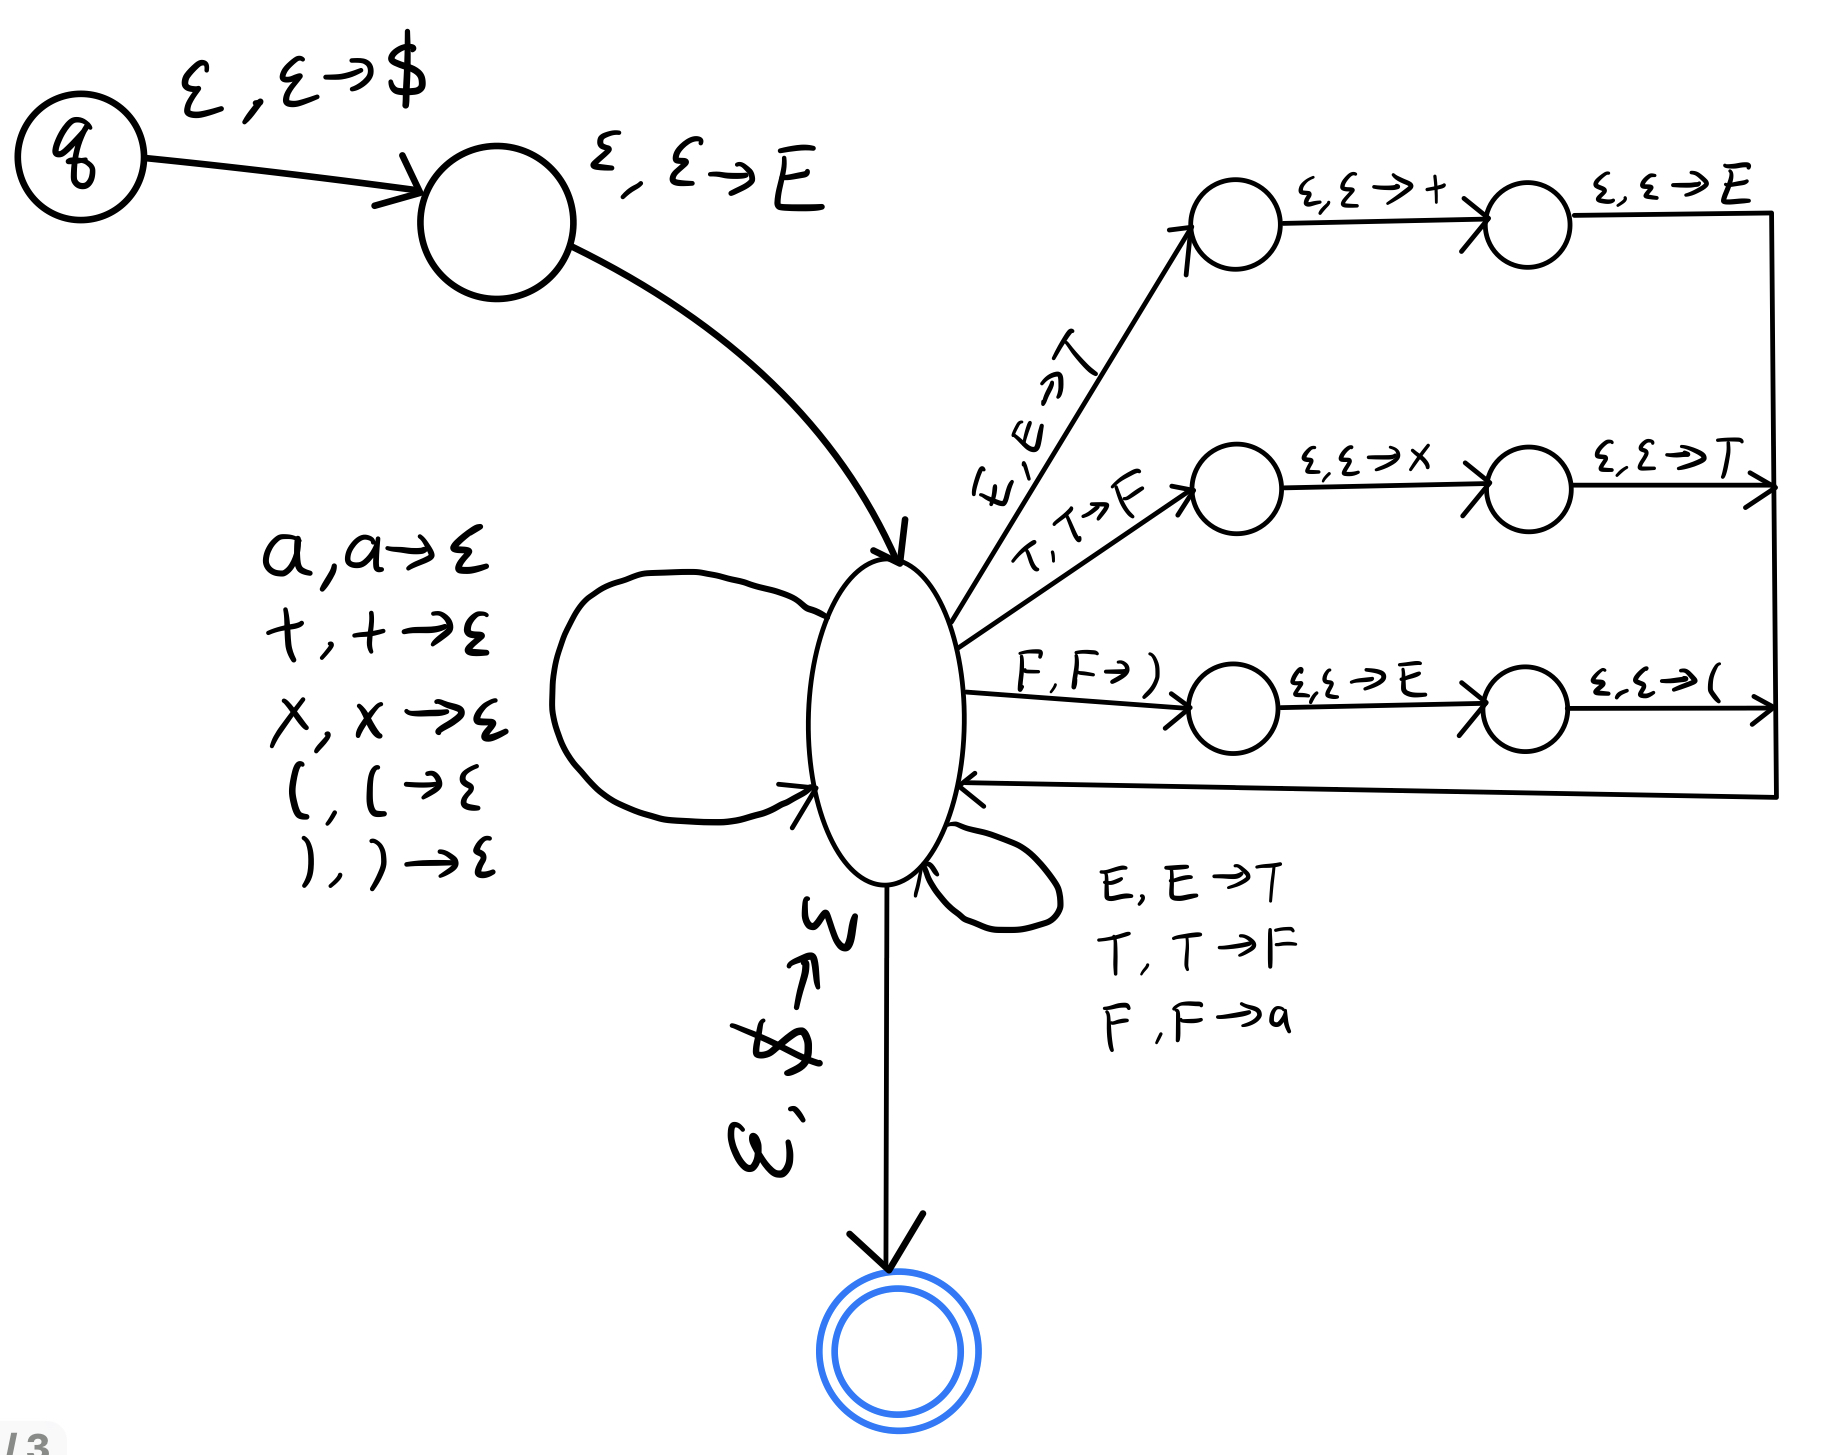
\includegraphics[width=7cm]{image/2.11.2.png}
        \caption{2.11}
        \label{fig:2_11}
    \end{figure}
\end{solution}






\textbf{第2.3次作业: 2.44, 2.2. 选做2.37.}

\problem{2.44} 对于字母表$\Sigma = \{1,2,3,4\}$上的语言$C=\{\omega\in \Sigma^* \mid \text{在}\omega\text{中, 1与2的个数相同, 3与4的个数相同}\}$,证明$C$不是上下文无关语言.


\begin{proof}
    使用关于上下文无关语言的泵引理进行反证. 假设$C$是上下文无关语言, 那么$\exists\,p \in \Z^+$,使得$C$中任何一个长度不小于$p$的宇符串$s$都能被划分成$5$段$s=uvxyz$, 且满足下述条件:
    \begin{enumerate}
        \item $\forall\,i\geq 0$, $uv^i xy^iz \in C$;
        \item $|vy| > 0$;
        \item $|vxy| \leq p$.
    \end{enumerate}

    由于语言的约束, 必须有$vy$中$1$与$2$的个数相等, 且$3$与$4$的个数相等. 构造字符串形式为$1^{p+1}3^{p+1}2^{p+1}4^{p+1} \in C$, 但无论如何使用分段方法与之匹配, 由于$|vxy| \leq p$的限制存在, $vxy$中至多存在$2$个不同的字符, 且一定是以下五种形式之一: $1^m$, $1^m3^n$, $3^m2^n$, $2^m4^n$, $4^m$. 无论哪一种可能性, 作为其中的两个子串, $v, y$永远不可能满足$vy$中$1$与$2$、$3$与$4$的个数相等 (因为母串中不可能同时存在每一对中的两种字符!), 因此无法找出$s=uvxyz$, 矛盾! 所以$C$不是上下文无关语言.
\end{proof}


\problem{2.2}

\problem{a.} 利用语言$A = \{a^m b^n c^n \mid m,n \geq 0\}$和$B = \{a^n b^n c^m \mid m,n \geq 0\}$以及例2.20, 证明上下文无关语言类在交运算下不封闭.

\begin{proof}
    考虑$A$与$B$的交集: $A \cap B =: C = \{a^n b^n c^n \mid n \geq 0\}$. 这很好理解, 因为$A, B$描述的均是$a,b,c$按顺序出现的字符串, 语言$A$中$b,c$的字数相同, 语言$B$中$a,b$的字数相同, 所以语言$C = A \cap B$中$a,b,c$的字数都相同. 接下来需要证明的是: $A,B$均为上下文无关语言, 而$C$不是. 证明使用关于上下文无关语言的泵引理.

    $A = \{a^m b^n c^n \mid m,n \geq 0\}$中任取字符串都有$a^m b^n c^n$的形式, 只需要取$u = a^mb^{n-1}, v = b, x = \varepsilon, y = c, z = c^{n-1}$, 这样$uv^i xy^iz = a^m b^{n+i-1} c^{n+i-1} \in C$. 这只需要$p=2$即可.
    
    $B = \{a^n b^n c^m \mid m,n \geq 0\}$中任取字符串都有$a^n b^n c^m$的形式, 只需要取$u = a^{n-1}, v = a, x = \varepsilon, y = b, z = b^{n-1}c^m$, 这样$uv^i xy^iz = a^{n+i-1} b^{n+i-1} c^m \in C$. 这只需要$p=2$即可.
    
    $C = \{a^n b^n c^n \mid n \geq 0\}$的情况则有不同. 假设其为上下文无关语言, 那么$\exists\,p$满足其条件; 这时取$s = a^p b^p c^p$, 发现无论如何取长度不超过$p$的子串, 总是只能包含$\{a,b,c\}$中的最多两个字符, 这样在将$v,y$乘幂叠加之后, 必然会产生$a,b,c$个数不相等的字符串 (比如$uv^2xy^2z \notin C$). 所以$C$不是上下文无关语言.

    $A \cap B \neq C$, 因此上下文无关语言类在交运算下不是封闭的.
\end{proof}

\problem{b.}利用 (a) 和德·摩根律 (定理0.10), 证明上下文无关语言类在补运算下不封闭.

\begin{proof}
    假设上下文无关语言类在补运算下封闭. 记上下文无关语言类为$S$, 已知$S$在并运算下封闭 (作为引理, 下面证明). 那么根据上一问的结果, 我们得到$A,B \in S$的交$C \notin S$. 因此有: $C = A \cap B = \overline{\overline{A \cap B}} = \overline{\overline{A} \cup \overline{B}}$. 然而, 
    $A,B \in S \Longrightarrow \overline{A}, \overline{B} \in S \Longrightarrow \overline{A} \cup \overline{B} \in S \Longrightarrow C = \overline{\overline{A} \cup \overline{B}} \in S$, 产生矛盾! 因此假设不成立, 上下文无关语言类在补运算下不封闭.

    现在证明引理: 上下文无关语言类在并运算下封闭. 每一个CFL都有一个CFG可以生成它, 对任意的两个初始CFL: $A, B$, 可以找出两个CFG: 
    $G_A = \{ V_A, \Sigma_A, R_A, S_A \}, G_B = \{ V_B, \Sigma_B, R_B, S_B \}$分别接受它们. 不妨令$V_A \cap V_B = \varnothing, \Sigma_A \cap \Sigma_B = \varnothing$. 构造一个新的CFG: 
    $G_C = \{ V_A \cup V_B \cup \{S_C\},\ \Sigma_A \cup V_C,\ R_A \cup R_B \cup \{S_C \rightarrow S_A \mid S_B\},\ S_C  \}$, 其中 $S_C \notin V_A \cup V_B$. 这样, 由于新的起始变元一定会生成$G_A,G_B$两种文法的起始变元之一, 且规则没有任何重叠, 我们可以得知这个文法生成的语言一定是原本两种文法生成的语言的并集, 即$G_C = G_A \cup G_B$, 引理得证.
\end{proof}



\problem{选做2.37} 对任一语言$A$, 令运算符$\operatorname*{SUFFIX}(A) = \{ v \mid \text{存在串}u, \text{使} uv\in A \} $, 证明上下文无关语言类在$\operatorname*{SUFFIX}$运算下封闭.

\begin{proof}
    对语言$A$, 可以找到一个满足乔姆斯基范式的上下文无关文法生成之, 记该文法为$G_A = \{ V, \Sigma, R, S \}$. 为其中每一条形如$V \rightarrow CD$的规则进行对应的规则新增: $V' \rightarrow C'D \mid CD \mid D \mid \omega$, 并将初始变元$S$改为$S'$. 概括性的叙述, 即含 "$'$" 的变元 (对应原本存在的每一条规则) 可以进行上述四种情形的替换, 而原本的变元依旧只能进行原本的替换. 这样, 对于一个原本存在的派生树, 我们能在某个特殊的时间节点将之最左侧 (始终只存在一个的) 含 "$'$" 的新变元抹去, 产生的字符串的最左侧一段 (可以是$\omega$) 也随之截去. 证明这样产生的新文法 (记作$G_A'$) 可以产生的语言即为$\operatorname*{SUFFIX}(A)$. 方法即使用二叉派生树对字符串$uv$进行分解, 分两个方向进行证明.

    (由于这是选做题, 就懒得写了, 以后有空的时候再打磨一下细节)
\end{proof}




\end{document}
